\documentclass{article}
\usepackage[T1]{fontenc}
\usepackage{iclr2027_conference,times}

\usepackage{hyperref}
\usepackage{url}
\usepackage{graphicx}
\usepackage{booktabs}
\usepackage{amsmath}
\usepackage{amssymb}
\usepackage{amsthm}
\usepackage{multirow}
\usepackage{array}
\usepackage{wrapfig}
\usepackage{colortbl}
\usepackage{enumitem}
\usepackage{placeins}
\usepackage{caption}
\usepackage{microtype}

\newcommand{\PreserveBackslash}[1]{\let\temp=\\#1\let\\=\temp}
\newcolumntype{C}[1]{>{\PreserveBackslash\centering}p{#1}}

\setlength{\textfloatsep}{11pt plus 2pt minus 2pt}
\setlength{\floatsep}{11pt plus 2pt minus 2pt}
\setlength{\intextsep}{11pt plus 2pt minus 2pt}
\setlength{\abovecaptionskip}{4pt}
\setlength{\belowcaptionskip}{2pt}
\renewcommand{\floatpagefraction}{0.85}

\theoremstyle{definition}
\newtheorem{property}{Property}

\title{MASOpt: Online Prompt Optimization for\\ Multi-Agent Systems with Closed-Loop Control}

\author{Anonymous Authors}

\begin{document}

\maketitle

\begin{abstract}
Large language model (LLM)-based multi-agent systems (MAS) decompose a complex task across specialized agents, where the prompt of each agent governs both its own behavior and the information it passes downstream. Existing MAS prompt optimizers search for a configuration before deployment and keep it fixed, which is an open-loop controller that never measures what its own output produces. In this paper, we introduce MASOpt, an online prompt optimization framework that closes this loop with the feedback principle of classical control theory. MASOpt treats the target MAS as a controlled plant and every local prompt edit as a control input whose value is determined only after the plant responds. A trajectory observer estimates a latent failure state from the partial execution, a minimal actuation module turns that state into a local prompt repair, and a feedback gate admits the repair only when the measured error decreases, so the retained prompt state never increases that error. To decide where to actuate instead of where the error becomes visible, we further propose Cross-Actuation Relative Advantage (CARA), which replays candidate actuations from an identical prefix and scores each against the others issued from the same state. Experiments on eight benchmarks show that MASOpt improves the average score from 80.58 to 83.40 over the strongest offline MAS prompt optimizer and raises the average interactive success rate from 39.23 to 64.85, with the backbone LLMs and the workflow topology left unchanged.
\end{abstract}

\section{Introduction}
\label{sec:introduction}

Large language model (LLM)-based multi-agent systems (MAS) have become a promising paradigm for tasks that exceed the reach of a single model call \citep{wu2023autogen,li2023camel,chen2023agentverse,yao2024multiagent}. By assigning planning, reasoning, execution, and verification to specialized agents \citep{li2023camel,chen2023agentverse}, a MAS decomposes a hard problem into coordinated sub-processes and aggregates the strengths of many LLM invocations \citep{wu2023autogen,zhang2024aflow}. Within such a system the prompt of each agent specifies its behavior, since it determines how the agent reads its role, consumes upstream messages, and hands information downstream \citep{khattab2024dspy,yuksekgonul2024textgrad}. Optimizing these prompts has therefore become the dominant mechanism for improving a MAS whose backbone models and topology are fixed \citep{mapro2026,hong2026maspob,wang2026maspo}. However, every prompt such an optimizer returns is committed before the task it must solve has started.

Unlike a single-agent prompt, which affects one output, a MAS prompt propagates along the topology, so an edit to an upstream agent changes the input distribution of every downstream agent it feeds \citep{mapro2026,wang2026maspo}. Prompt quality is therefore a property of the execution state, not of the prompt. An instruction that steers a solver correctly at the start of a derivation turns harmful once the solver emits a malformed expression, because the downstream verifier inherits it and spends the remaining budget confirming it \citep{hendrycks2021math}. The effect is considerably sharper in long-horizon interaction, where one misread dependency propagates through the remaining steps of a 20-step TextCraft episode and a configuration fixed beforehand cannot intervene at the third step even though the failure is already visible \citep{prasad2024textcraft}. In both cases the evidence needed to fix the prompt arrives while the prompt is already in use, and an optimizer that has finished its work cannot read it.

Existing MAS prompt optimization can be broadly categorized into agent-wise and system-level optimization. Early efforts optimize each agent independently with a generic prompt optimizer \citep{zhou2022ape,pryzant2023automatic,yang2024opro,fernando2024promptbreeder,lin2023instinct}, treating the remaining agents as a static environment. However, these methods ignore the dependencies the topology induces, so a locally improved prompt can still degrade the workflow containing it \citep{mapro2026}. More recently, a line of work models the interaction among prompts explicitly through topology-aware feedback, budget-constrained black-box search, or downstream-utility scoring \citep{mapro2026,hong2026maspob,wang2026maspo}. Although these systems capture the coupling far better, each still returns one configuration frozen at deployment \citep{zhang2024aflow,xia2025hivemind}. In essence, both categories are open-loop, as they compute a control sequence in advance and apply it without measuring what it produces.

\begin{figure}[t]
    \centering
    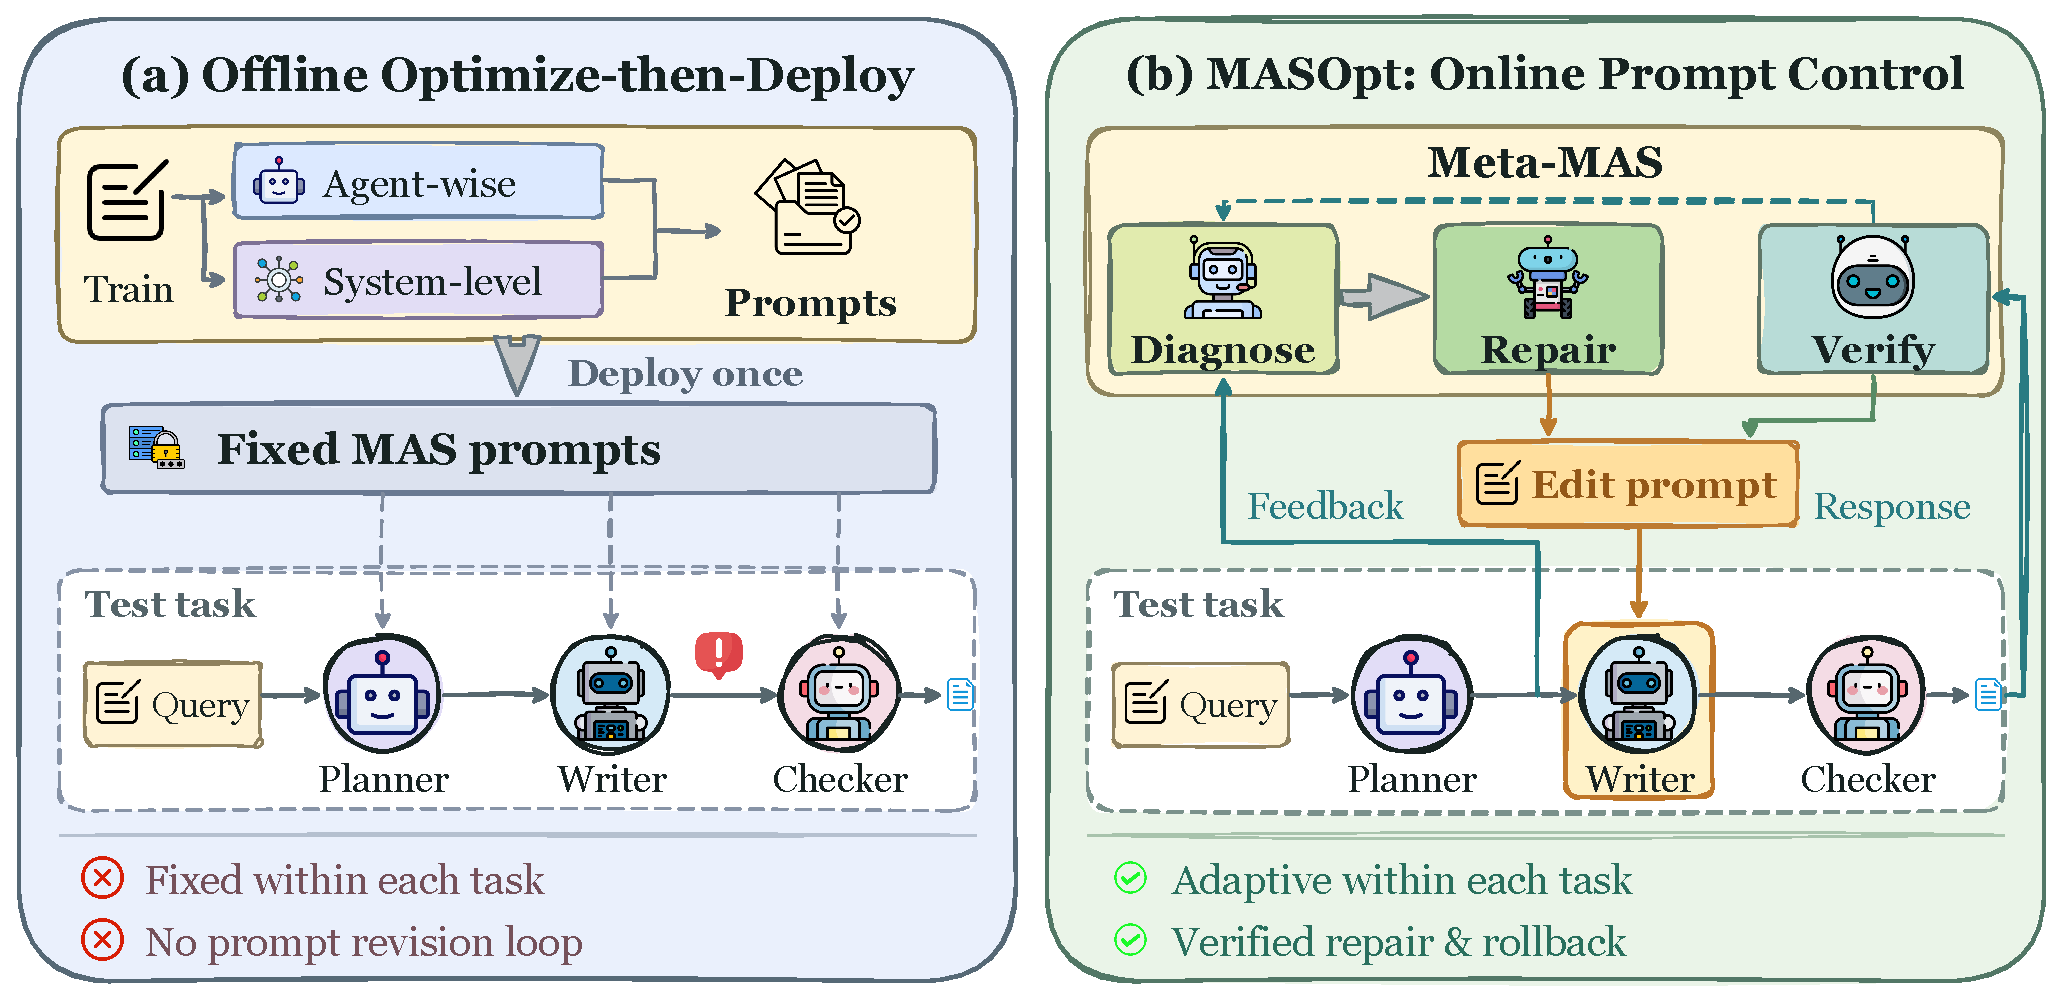
\includegraphics[width=0.74\linewidth]{figures/masopt_introduction_comparison.pdf}
    \caption{Offline prompt optimization is an open-loop controller that commits a configuration before execution, while MASOpt closes the loop inside the episode and keeps a local prompt repair only when the measured error decreases.}
    \label{fig:masopt-paradigms}
\end{figure}

In this paper, we aim to advance MAS prompt optimization from open loop to closed loop. Classical control theory establishes that an open-loop controller reaches the intended behavior only when the plant model is exact and no disturbance enters the loop, and that feedback is what lets a controller tolerate both \citep{astrom2008feedback,goodwin2001control}. An LLM-based MAS satisfies neither condition. Its response to a prompt is unpredictable, and every task instance injects a different disturbance. Along with this idea, we propose \emph{MASOpt}, which treats the target MAS as the controlled plant, the observable trajectory as the measurement, and each local prompt edit as a control input. Figure~\ref{fig:masopt-paradigms} contrasts the two regimes. Specifically, to recover the failure a measurement reveals only partially, MASOpt introduces a \emph{trajectory observer} that estimates a latent failure state. To act on that state without disturbing the workflow, MASOpt restricts the control input to a \emph{minimal actuation} on one agent or one interface, keeping the perturbation small enough for its effect to be attributed. To stop an unverified edit from corrupting the episode, a \emph{feedback gate} admits an actuation only when the measured error decreases and reverts it otherwise. This revert branch is what separates a controller from iterative self-refinement, since Self-Refine rewrites an output and Reflexion accumulates a memory for the next trial, while neither can withdraw a change that made the system worse \citep{madaan2023selfrefine,shinn2023reflexion}.

Closing the loop still leaves open where to actuate. In a MAS the agent at which an error becomes visible is frequently not the agent at which actuation is most effective, since the error is produced upstream and only surfaces downstream \citep{mapro2026}. To resolve this, we propose \emph{Cross-Actuation Relative Advantage} (CARA), which replays every candidate actuation from an identical saved prefix and scores it against the others issued from the same state. Fixing the prefix removes the confound of a different preceding trajectory, so the comparison isolates the actuation itself, in the same way that a step response is interpretable only from a known initial condition \citep{astrom2008feedback,goodwin2001control}. The resulting preferences form a frozen \emph{feedback control memory} that the controller queries as a prior, which lets the loop settle within a few rounds instead of exploring at test time.

Experiments on eight benchmarks covering code generation \citep{chen2021humaneval,austin2021mbpp}, mathematical reasoning \citep{cobbe2021gsm8k,hendrycks2021math}, reading comprehension \citep{yang2018hotpotqa,dua2019drop}, and interactive decision making \citep{shridhar2020alfworld,prasad2024textcraft} show that MASOpt improves the average score from 80.58 to 83.40 over MASPOB \citep{hong2026maspob} and the average interactive success rate from 39.23 to 64.85. In summary, our key contributions are three-fold.
\begin{itemize}[leftmargin=1em, itemsep=-1ex, topsep=0ex]
    \item \textbf{Closed-Loop Formulation.} To the best of our knowledge, MASOpt is the first framework that formulates MAS prompt optimization as closed-loop control, where measurements taken inside an episode determine the prompts governing the remainder of that same episode.
    \item \textbf{Verified Actuation with CARA.} We build a controller from a trajectory observer, a minimal actuation module, and a feedback gate that guarantees a monotone measured error, and propose Cross-Actuation Relative Advantage to learn where to actuate from matched-state replay.
    \item \textbf{Strong Performance.} Experiments on eight benchmarks show that MASOpt outperforms the strongest offline MAS prompt optimizer by 2.82 points on average and by 25.62 points on interactive success.
\end{itemize}

\section{Related Work}
\label{sec:related_work}

\textbf{Automatic Prompt Optimization}\quad The sensitivity of LLMs to natural-language instructions has motivated a broad line of work on automatic prompt optimization. Early approaches select instruction candidates through task-level evaluation \citep{zhou2022ape,pryzant2023automatic}, OPRO casts optimization as a language modeling problem \citep{yang2024opro}, and PromptBreeder evolves the task prompts together with the mutation prompts that modify them \citep{fernando2024promptbreeder,lin2023instinct}. Another group optimizes structured language-model programs, where DSPy compiles prompts as pipeline parameters \citep{khattab2024dspy}, TextGrad propagates textual feedback in analogy with automatic differentiation \citep{yuksekgonul2024textgrad,agrawal2025textgrad}, and SkillOpt treats agent skills the same way \citep{yang2026skillopt}. However, all of these optimizers collect their signal at the level of a complete trial, so they learn that a prompt is bad without learning at which point of the trajectory it became bad.

\textbf{System-Level Prompt Optimization for Multi-Agent Systems}\quad Prompt optimization is substantially harder in a MAS, because prompts interact through the topology and improving one agent in isolation changes what every downstream agent receives \citep{wu2023autogen,li2023camel}. MAPRO casts the problem as maximum a posteriori inference with topology-aware feedback \citep{mapro2026}, MASPOB as budget-constrained black-box search with a graph neural surrogate \citep{hong2026maspob}, and MASPO scores a prompt by its contribution to downstream success \citep{wang2026maspo}. A further line searches the structure of the workflow itself \citep{zhang2024aflow,xia2025hivemind,zhao2025a2flow}. Overall, these methods establish that MAS prompts must be optimized as a coupled system, yet their optimization target remains a configuration selected before deployment.

\textbf{Runtime Feedback and Online Adaptation}\quad A related line studies how language agents improve from feedback at test time. Self-Refine alternates between feedback generation and output refinement \citep{madaan2023selfrefine,pan2024critic}, Reflexion converts environmental feedback into verbal reflections kept in an episodic memory \citep{shinn2023reflexion,yao2023react}, and MemRL learns utilities over such memories while the base model stays fixed \citep{zhang2026memrl}. These studies establish the value of non-parametric adaptation, yet their adaptation target is either a single output or a memory consumed by the next episode.

In this work, we focus on the prompt state of a running multi-agent system, with the goal of letting measurements taken inside an episode determine the prompts that govern the remainder of that episode. Unlike previous approaches that treat a configuration as a parameter chosen before deployment, MASOpt adopts a more deliberate design by treating every prompt edit as a control input whose effect is measured from the response of the plant. An ineffective edit is reverted, and an unresolved failure triggers another round.

\section{MASOpt}
\label{sec:method}

We introduce MASOpt, an online prompt optimization framework that applies the feedback principle of classical control to a fixed multi-agent system. Because a plausible prompt edit may resolve the failure, do nothing, or create a new one downstream, MASOpt measures the response of the plant before deciding whether to keep it. The overview of MASOpt is illustrated in Figure~\ref{fig:masopt-overview}, and its formulation, controller, offline calibration, and online loop are introduced as follows.

\begin{figure}[t]
    \centering
    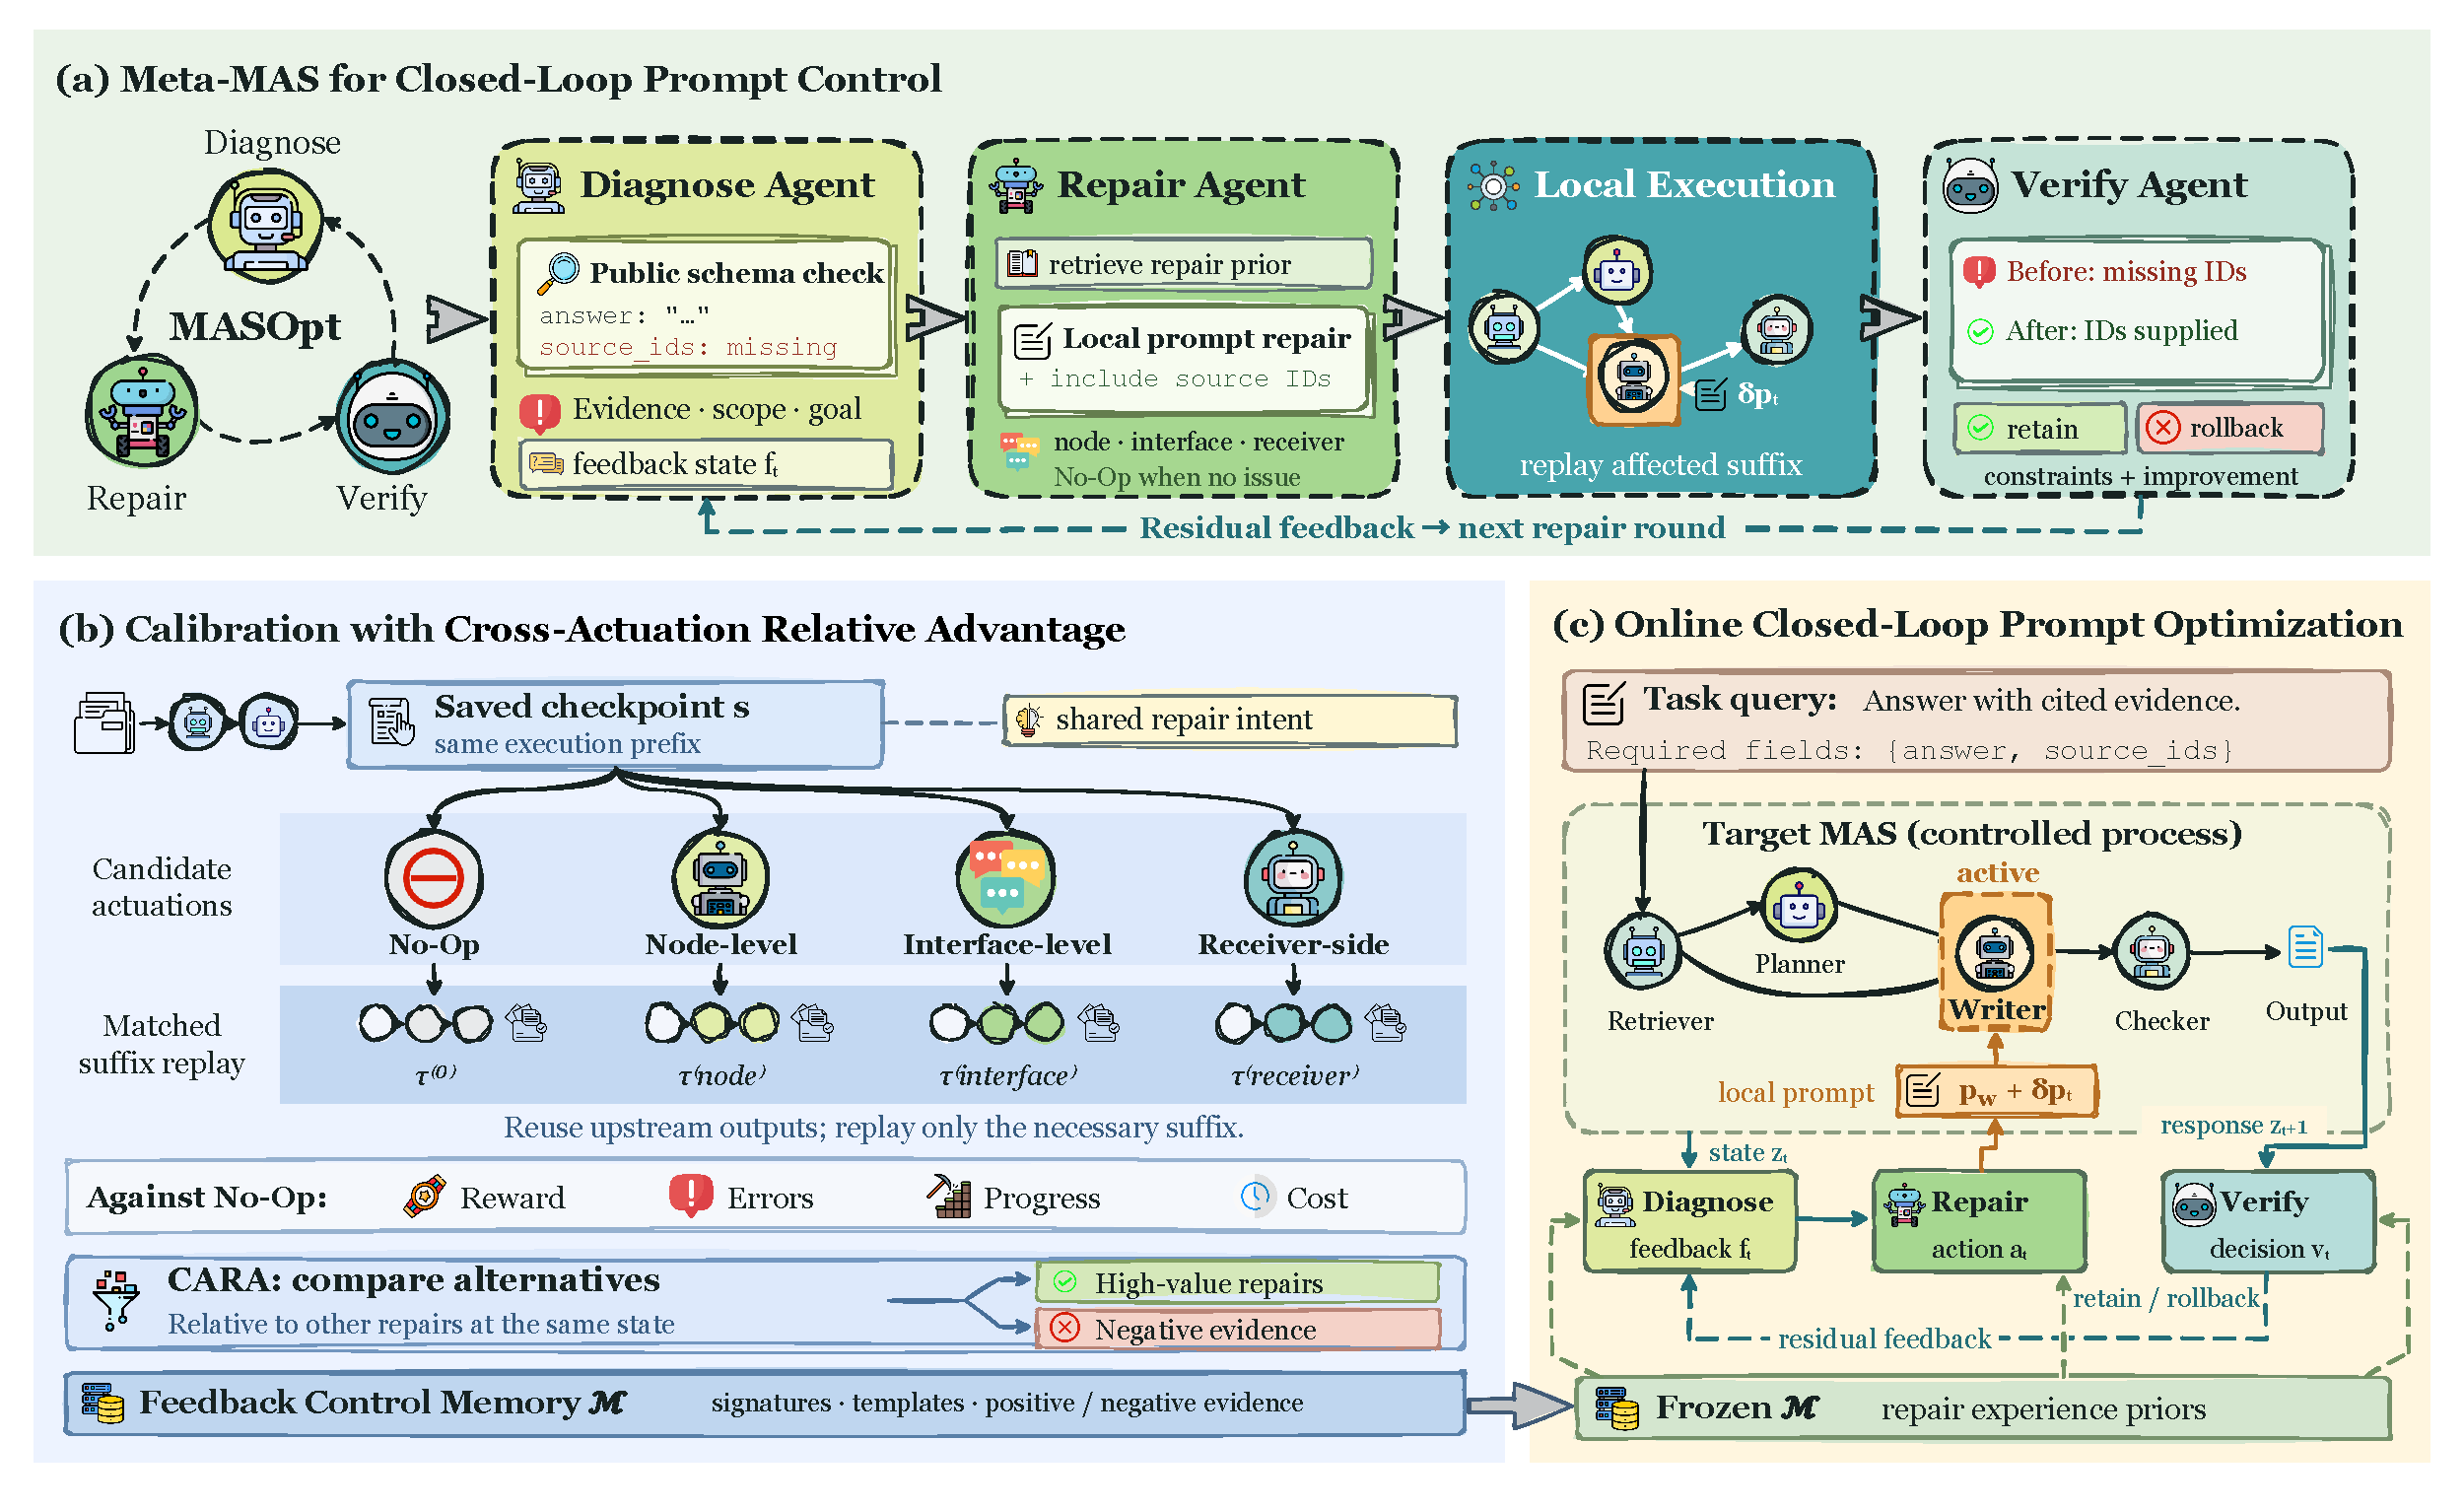
\includegraphics[width=0.80\linewidth]{figures/masopt_method_overview.pdf}
    \caption{Overview of MASOpt. \textbf{(a)} The controller estimates a latent failure state, actuates a minimal prompt repair, and admits it through a feedback gate. \textbf{(b)} CARA replays candidate actuations from an identical prefix and distills their relative advantage into a feedback control memory. \textbf{(c)} At deployment the memory is frozen and every actuation is retained or reverted by the measured response.}
    \label{fig:masopt-overview}
\end{figure}

\subsection{From Open-Loop to Closed-Loop Prompt Optimization}
\label{sec:problem}

\textbf{Plant, Measurement, and Control Input}\quad We consider a fixed multi-agent workflow $\mathcal{G}=(\mathcal{V},\mathcal{E})$, where each node is an agent invocation and each edge carries information from an upstream agent to a downstream one \citep{zhang2024aflow}. The topology and the backbone LLMs stay fixed \citep{hong2026maspob}, and the only quantity a controller may change is the prompt state $\mathbf{P}_t = ( p^{t}_{1}, \cdots, p^{t}_{N} )$ of the $N$ agents, with $\mathbf{P}_0$ the deployed configuration. For a task $x$ the plant emits a partial trajectory $\tau_t$ of responses, inter-agent messages, tool results, and environment observations, of which the controller sees only the measurement $z_t = f_{\mathrm{obs}}( x, \tau_t )$ that excludes hidden labels. A checkpoint is eligible once an agent has produced a complete output that a downstream agent or the environment will consume. At such a checkpoint the controller applies a control input $a_t \in \mathcal{A}(z_t)$, which we call an \emph{actuation}. It edits one agent instruction, one interface constraint, or one receiver-side rule, giving
\begin{gather}
    \mathbf{P}_{t+1} = f_{\mathrm{act}}\left( \mathbf{P}_t, a_t \right), \qquad e_t = \mathcal{E}\left( z_t \right), \label{eq:prompt_update}
\end{gather}
where $f_{\mathrm{act}}(\cdot)$ writes only the local modification $a_t$ specifies, and the \emph{measured error} $\mathcal{E}(\cdot)$ counts the label-free runtime violations the trajectory exposes, including failed public tests, unparsable outputs, missing message fields, unsatisfied dependencies, and invalid environment actions. Counting violations instead of estimating task reward is deliberate, since a violation cannot be traded against correctness. A no-operation input is always available.

\textbf{Open-Loop and Closed-Loop Objectives}\quad An offline optimizer solves the open-loop problem $\max_{\mathbf{P}} \mathbb{E}_{x \sim \mathcal{D}} [ R( \tau_T \mid \mathbf{P} ) ]$ once and applies the solution unchanged, with $R$ the final task metric over the task distribution $\mathcal{D}$ \citep{hong2026maspob,wang2026maspo}. MASOpt instead learns a policy $\pi$ that emits an actuation at every checkpoint,
\begin{gather}
    \max_{\pi} \; \mathbb{E}_{x \sim \mathcal{D}} \left[ R\left( \tau_T \right) - \lambda \sum\nolimits_{t=1}^{T} C\left( a_t \right) \right], \quad a_t \sim \pi \left( \cdot \mid x, z_{\leq t}, \mathcal{M} \right), \label{eq:objective}
\end{gather}
where $C(a_t)$ is the cost of an actuation, $\lambda$ trades control effort against task utility, and $\mathcal{M}$ is the calibrated experience obtained offline. The one difference that matters is that $a_t$ conditions on $z_{\leq t}$, which contains the measurements produced \emph{after} $a_{t-1}$ was applied. The formulation needs only the observable trajectory and a local edit, which lets it control a plant whose response cannot be modeled in advance.

\subsection{A Closed-Loop Controller over Prompt State}
\label{sec:meta_agents}

MASOpt realizes $\pi$ with three modules that mirror the observer, the actuator, and the feedback path of a regulator \citep{astrom2008feedback,goodwin2001control}. Separating estimation, actuation, and acceptance makes an effect attributable, since the module proposing an edit never decides whether it worked.

\textbf{Trajectory Observer for Latent Failure State}\quad A measurement reports the symptom of a failure, so the controller first estimates its cause. The trajectory observer maps the observable history and the retrieved experience to a structured latent failure state
\begin{gather}
    s_t = f_{\mathrm{diag}}\left( x, z_{\leq t}; \mathcal{M} \right), \label{eq:diagnose}
\end{gather}
where $s_t$ records the detected failure, its evidence, its severity, its scope, and the behavior to restore. MASOpt checks the deterministic signals before any semantic estimation, so a failed public test or an invalid environment action enters $s_t$ as hard evidence. The observer answers what must be corrected without committing to an edit, which leaves the actuation space free for the next module.

\textbf{Minimal Actuation for Local Prompt Repair}\quad Large edits are easy to propose and impossible to attribute. MASOpt therefore restricts the control input to the smallest local change that can plausibly remove the diagnosed failure,
\begin{gather}
    a_t = f_{\mathrm{rep}}\left( s_t, \mathbf{P}_t, z_t; \mathcal{M} \right), \label{eq:repair}
\end{gather}
where $f_{\mathrm{rep}}(\cdot)$ searches an action space of node-level edits, interface-level constraints, receiver-side rules, and the no-operation input. The retrieved experience supplies a prior over the actuation type, while the current context instantiates the text. MASOpt bounds the perturbation so that the effect of an actuation stays separable from the ordinary variance of the plant, which is what makes verification possible.

\textbf{Feedback Gate for Verified Acceptance}\quad MASOpt treats a proposed repair as a hypothesis, so it replays the affected part of the workflow to a comparable checkpoint and compares the new measurement against the pre-actuation one,
\begin{gather}
    g_t = f_{\mathrm{ver}}\left( s_t, z_t, z_{t+1}; \mathcal{M} \right), \label{eq:verify}
\end{gather}
where $g_t \in \{\textsc{Accept}, \textsc{Reject}\}$ carries the decision together with a description of whatever failure remains. The gate admits an actuation only when the measured error decreases and no hard constraint is violated, which yields the closed-loop update
\begin{gather}
    \mathbf{P}_{t+1} =
    \begin{cases}
        f_{\mathrm{act}}\left( \mathbf{P}_t, a_t \right), & \text{if } g_t = \textsc{Accept} \text{ and } \mathcal{E}(z_{t+1}) < \mathcal{E}(z_{t}), \\[2pt]
        \mathbf{P}_t, & \text{otherwise}.
    \end{cases}
    \label{eq:accept}
\end{gather}
The gate is what closes the loop. When an actuation removes only part of the failure, the residual enters the next latent state $s_{t+1}$ and drives another bounded round. This recursion separates MASOpt from one-shot prompt rewriting \citep{madaan2023selfrefine}, because the controller never assumes its first actuation was correct.

\begin{property}[Monotone measured error]
\label{prop:monotone}
Let $\tilde{e}_t$ denote the measured error evaluated at the prompt state MASOpt holds after the gate at checkpoint $t$. Under Equation~\ref{eq:accept} the sequence $\tilde{e}_0, \tilde{e}_1, \cdots, \tilde{e}_T$ is non-increasing, so the terminal prompt state satisfies $\tilde{e}_T \leq \tilde{e}_0$.
\end{property}

Neither an open-loop optimizer nor an iterative rewriter has this guarantee. The former never measures its own effect and the latter keeps whatever it produced last, so both can admit an edit that raises the error \citep{fernando2024promptbreeder,madaan2023selfrefine}. The guarantee holds independently of the observer and of the actuation module, which is the robustness that feedback buys over search \citep{astrom2008feedback}.

\subsection{Actuation Calibration with Cross-Actuation Relative Advantage}
\label{sec:cara}

A closed loop still has to choose where to act. With no prior it must find the right actuation by trial at deployment, which is costly and slow to settle. MASOpt therefore calibrates the actuation choice offline, with no LLM parameter updated.

\textbf{Matched-State Actuation Probing}\quad Comparing two actuations applied after different preceding trajectories confounds the effect of the actuation with the effect of the trajectory, so MASOpt replays every candidate from the same saved prefix. Specifically, for an informative checkpoint $s$ we construct a repair intent that states the behavior to restore without prescribing where to apply it, which yields $\mathcal{A}_s = \{ a_0, a_1, \cdots, a_K \}$ with $a_0$ the no-operation input and the remainder legal local actuations at different points of the workflow. MASOpt reuses the unaffected upstream outputs and replays only the necessary suffix, which turns each probe into a controlled response measurement from a known initial condition \citep{astrom2008feedback,goodwin2001control}.

\textbf{Cross-Actuation Relative Advantage}\quad For an actuation $a$ at state $s$, we first score the paired outcome against the matched no-operation replay,
\begin{gather}
    U(s,a) = \lambda_R \Delta R(s,a) + \lambda_E \Delta E(s,a) + \lambda_P \Delta P(s,a) - \lambda_C C(s,a), \label{eq:utility}
\end{gather}
where $\Delta R$ is the task-reward improvement over the matched no-operation, $\Delta E$ the reduction in observable execution error, $\Delta P$ the progress toward completion, and $C$ the actuation and replay cost. Absolute utility is not comparable across heterogeneous states, since an easy checkpoint rewards every candidate and a hopeless one rewards none. We therefore score each candidate against the others issued from the same state, which gives the Cross-Actuation Relative Advantage
\begin{gather}
    A_{\mathrm{CARA}}(s,a) = \frac{U(s,a) - \mu_{-a}(s)}{\sigma_{-a}(s) + \epsilon}, \quad \mu_{-a}(s) = \frac{1}{\left| \mathcal{A}_s \right| - 1} \sum\nolimits_{b \in \mathcal{A}_s, b \neq a} U(s,b), \label{eq:cara}
\end{gather}
where $\sigma_{-a}(s)$ is the standard deviation of $U(s,b)$ over the remaining candidates and $\epsilon$ stabilizes the ratio. Equation~\ref{eq:cara} takes the form of a leave-one-out group-relative advantage, with two differences. The group collects actuations applied at \emph{different points of one workflow} instead of repeated samples of one prompt, and the estimate is stored in a memory instead of a parameter update. CARA therefore measures whether an actuation is unusually effective \emph{for this execution state}, which is the question a MAS controller faces, because the node where an error becomes visible is often not the node where actuation has the largest effect \citep{mapro2026}.

\textbf{Feedback Control Memory}\quad MASOpt collects the calibrated preferences into a reusable memory $\mathcal{M}$, where each entry records a failure signature, the topology context, an actuation type, a bounded prompt template, and its effectiveness statistics. We keep the actuations of consistently negative advantage as negative evidence, since knowing which repair to avoid at a state removes exploration the online loop would otherwise pay for \citep{zhang2026memrl}. At deployment $\mathcal{M}$ is frozen, is queried only as a prior, and never stores task answers.

\subsection{Online Closed-Loop Optimization}
\label{sec:online}

At deployment MASOpt starts every task from $\mathbf{P}_0$ and the frozen $\mathcal{M}$, with no ground-truth answer available. The plant runs normally until an eligible checkpoint, and if the evidence indicates no meaningful failure then no actuation is applied, which keeps the control effort near zero on the tasks the system already solves. Otherwise the observer builds $s_t$, retrieves matching entries from $\mathcal{M}$, and the actuation module instantiates a minimal edit applied only to the affected part of the workflow, reusing the unaffected upstream computation whenever the environment supports checkpoint replay. The gate then evaluates the post-actuation measurement from runtime signals alone, and Equation~\ref{eq:accept} retains or reverts the prompt state. The loop stops when the residual is empty, when the gate rejects every candidate, or when the round budget is exhausted. Every actuation is cleared at termination, so MASOpt adapts within a task while the target models, the topology, and the cross-task memory stay fixed, which is the opposite of a memory that accumulates across episodes \citep{shinn2023reflexion,zhang2026memrl}.

\section{Experiments}
\label{sec:experiments}

We evaluate whether closing the loop inside an episode still improves a multi-agent system that a strong offline optimizer has already tuned.

\subsection{Experimental Setting}
\label{sec:experimental-setup}

\textbf{Benchmarks}\quad We evaluate MASOpt on eight benchmarks covering code generation \citep{chen2021humaneval,austin2021mbpp}, mathematical reasoning \citep{cobbe2021gsm8k,hendrycks2021math}, reading comprehension \citep{yang2018hotpotqa,dua2019drop}, and interactive decision making \citep{shridhar2020alfworld,prasad2024textcraft}. Benchmark details refer to Appendix~\ref{app:data-splits}.

\textbf{Baselines}\quad We compare MASOpt with reasoning-based prompting \citep{wei2022cot,yao2023react}, prompt optimization \citep{fernando2024promptbreeder,lin2023instinct,opsahlong2024mipro,hong2026maspob}, and workflow generation \citep{zhang2024aflow,xia2025hivemind}. MASPOB is the strongest published system-level MAS prompt optimizer \citep{hong2026maspob}, and baseline results on the six non-interactive benchmarks follow its evaluation setting. Detailed description of baselines refer to Appendix~\ref{app:protocols}.

\textbf{Configuration}\quad Unless otherwise stated, every agent of the target MAS is served by \texttt{gpt-4o-mini} with temperature $0$ and top-$p$ $1$, and the backbone parameters stay frozen \citep{yang2026skillopt}. Specifically, MASOpt runs on the same locally executed workflow as the within-system baselines, so the topology, the roles, and $\mathbf{P}_0$ are identical across arms. Ground-truth rewards enter only the offline utility of Equation~\ref{eq:utility} and are never exposed to the online gate. Interactive runs use a $35$-step limit on ALFWorld and a $20$-step limit on TextCraft with at most two actuation rounds per checkpoint. We report pass@1 on the code benchmarks, accuracy on the mathematical ones, F1 on the reading benchmarks, and success rate on the interactive ones. Further details refer to Appendix~\ref{app:impl}.

\subsection{Main Results}
\label{sec:main-results}

\begin{table}[t]
    \centering
    \caption{Performance (\%) on six non-interactive benchmarks. Baselines are ordered by increasing average and MASOpt is separated at the bottom. `Avg.' is the unweighted six-benchmark mean and the best results are marked in \textbf{bold}.}
    \label{tab:main-results}
    \small
    \setlength{\tabcolsep}{5pt}
    \begin{tabular}{@{}lccccccc@{}}
        \toprule
        \textbf{Method} & \textbf{HumanEval} & \textbf{MBPP} & \textbf{GSM8K} & \textbf{MATH} & \textbf{HotpotQA} & \textbf{DROP} & \textbf{Avg.} \\
        \midrule
        \textbf{IO} & 89.31 & 69.11 & 87.80 & 51.71 & 60.36 & 53.09 & 68.56 \\
        \textbf{CoT} & 89.57 & 69.89 & 88.34 & 52.47 & 67.62 & 58.27 & 71.03 \\
        \textbf{ReAct} & 87.79 & 66.08 & 88.91 & 52.61 & 65.61 & 67.25 & 71.38 \\
        \textbf{PromptBreeder} & 88.80 & 70.38 & 91.97 & 52.13 & 68.76 & 71.85 & 73.98 \\
        \textbf{Instinct} & 90.08 & 70.23 & 92.64 & 52.40 & 69.92 & 71.90 & 74.53 \\
        \textbf{HiveMind} & 89.31 & 71.55 & 92.99 & 57.41 & 67.23 & 68.76 & 74.54 \\
        \textbf{AFlow} & 91.09 & 79.96 & 93.36 & 53.83 & 73.42 & 79.48 & 78.52 \\
        \textbf{MIPRO} & 91.35 & 80.65 & 92.80 & 54.90 & 74.37 & 79.13 & 78.87 \\
        \textbf{MASPOB} & 94.15 & 80.65 & 93.90 & 57.05 & 75.43 & 82.28 & 80.58 \\
        \midrule
        \rowcolor{gray!15}\textbf{MASOpt} & \textbf{96.95} & \textbf{84.16} & \textbf{94.41} & \textbf{62.76} & \textbf{76.49} & \textbf{85.66} & \textbf{83.40} \\
        \bottomrule
    \end{tabular}
\end{table}

\textbf{Capability on Program Synthesis and Mathematical Reasoning}\quad We evaluate MASOpt on HumanEval, MBPP, GSM8K, and MATH to assess its \emph{verifiable reasoning capabilities}, where every intermediate failure leaves an executable trace a controller can measure without labels. We compare with PromptBreeder \citep{fernando2024promptbreeder}, Instinct \citep{lin2023instinct}, MIPRO \citep{opsahlong2024mipro}, AFlow \citep{zhang2024aflow}, and MASPOB \citep{hong2026maspob} on the same backbone. As shown in Table~\ref{tab:main-results}, MASOpt outperforms MASPOB by 2.80 and 3.51 points on the two code benchmarks and substantially by 5.71 points on MATH. The size of each gain tracks how much room a task leaves for repair, since GSM8K already saturates at 93.90 under the offline optimizer while MATH carries the longest derivations and gains the most. An offline optimizer cannot produce this pattern, because it applies the same instruction to a saturated task and to an unsaturated one, while MASOpt spends an actuation only where a trajectory exposes a failure. Overall, these results highlight that a measurable runtime error signal is what turns a fixed prompt configuration into a correctable one.

\textbf{Capability on Multi-Hop and Discrete Reasoning}\quad We further evaluate MASOpt on HotpotQA and DROP to assess its \emph{evidence-grounded reasoning capabilities}, where a failure is an incomplete aggregation of retrieved evidence instead of a hard execution error. We compare against the same baselines under the identical workflow. As shown in Table~\ref{tab:main-results}, MASOpt improves over MASPOB by 1.06 and 3.38 points. Notably, the asymmetry between the two benchmarks is informative, since DROP failures surface as arithmetic and span-selection violations that the observer detects directly, while HotpotQA failures are semantic and leave a particularly weak label-free signal \citep{yang2018hotpotqa,dua2019drop}. The formulation predicts this dependence, since the strength of the feedback signal bounds how much a controller can repair. Overall, these results highlight that MASOpt converts observable constraint violations into targeted prompt repairs.

\begin{wraptable}{r}{0.49\textwidth}
    \centering
    \caption{Interactive success rate (\%) under the shared action interface and the identical step limits. `Avg.' weights the three score columns equally and the best results are marked in \textbf{bold}.}
    \label{tab:interactive-results}
    \small
    \setlength{\tabcolsep}{4pt}
    \begin{tabular}{@{}lcccc@{}}
        \toprule
        & \multicolumn{2}{c}{\textbf{ALFWorld}} & & \\
        \cmidrule(lr){2-3}
        \textbf{Method} & \textbf{Seen} & \textbf{Unseen} & \textbf{TextCraft} & \textbf{Avg.} \\
        \midrule
        \textbf{HiveMind} & 28.57 & 27.61 & 12.50 & 22.89 \\
        \textbf{MASPOB} & 47.86 & 50.75 & 13.75 & 37.45 \\
        \textbf{MIPRO} & 51.43 & 50.00 & 12.50 & 37.98 \\
        \textbf{AFlow} & 50.71 & 54.48 & 12.50 & 39.23 \\
        \midrule
        \rowcolor{gray!15}\textbf{MASOpt} & \textbf{75.00} & \textbf{89.55} & \textbf{30.00} & \textbf{64.85} \\
        \bottomrule
    \end{tabular}
\end{wraptable}

\textbf{Capability on Long-Horizon Interactive Decision Making}\quad We evaluate MASOpt on ALFWorld and TextCraft to assess its \emph{long-horizon recovery capabilities}, where an early mistake compounds over the remaining steps and no single final answer exists. We compare with the same baselines under the shared typed action interface and the identical step limits. As shown in Table~\ref{tab:interactive-results}, MASOpt solves 24 of 80 TextCraft tasks and significantly lifts the three-column average from 39.23 to 64.85. This margin is far larger than on the non-interactive benchmarks, which follows from the formulation, since an interactive episode emits a dense stream of dependency and inventory violations the observer reads at every step while a single-turn task emits one measurement at the end. The unseen split gains more than the seen split for the same reason, because an unfamiliar layout produces more invalid actions for the observer to read. Overall, the benefit of closing the loop grows with the number of measurements the plant makes available.

\section{Analyses}
\label{sec:analyses}

Each study below tests a prediction that the formulation makes, asking in turn whether the closed loop depends on its calibrated experience, whether it improves the instructions themselves, and whether it survives a change of workflow architecture and of backbone model.

\subsection{Effect of Diagnostic and Verification Experience}
\label{sec:experience-ablation}

\begin{figure}[t]
    \centering
    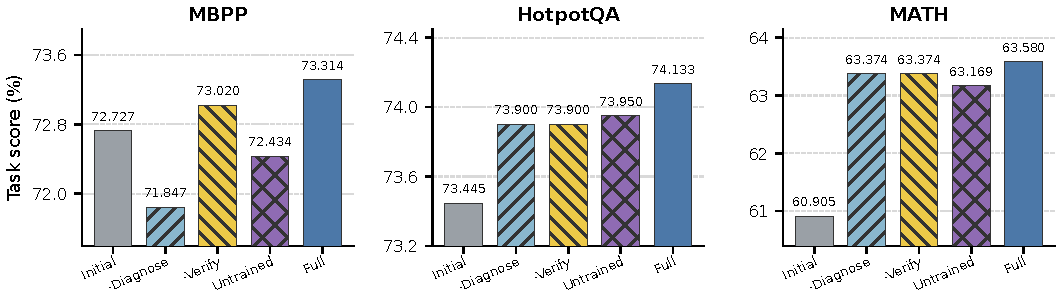
\includegraphics[width=0.95\textwidth]{figures/ablation_experience.pdf}
    \caption{Experience ablations on MBPP, HotpotQA, and MATH. Each panel compares the full controller with the variants that remove diagnostic experience, verification experience, or all learned experience, where every arm reuses the same Initial outputs.}
    \label{fig:experience-ablation}
\end{figure}

The feedback control memory is central to MASOpt, as it supplies the prior that keeps the online loop short. To investigate its effect, we conduct an ablation study that removes the calibrated experience from the observer, from the gate, and from both, while the controller and the workflow stay unchanged. As shown in Figure~\ref{fig:experience-ablation}, the full controller is the strongest arm on all three benchmarks. In particular, the ordering among the ablations locates the bottleneck of the loop in state estimation. Removing diagnostic experience is the most damaging setting, since an actuation aimed at a misidentified failure cannot reduce the measured error however well the gate is calibrated. Removing verification experience is milder, because the gate retains the deterministic runtime constraints. Overall, the calibrated prior removes the exploration that the loop would otherwise pay for at deployment \citep{zhang2026memrl}.

\begin{figure}[t]
    \centering
    \begin{minipage}[b]{0.285\textwidth}
        \centering
        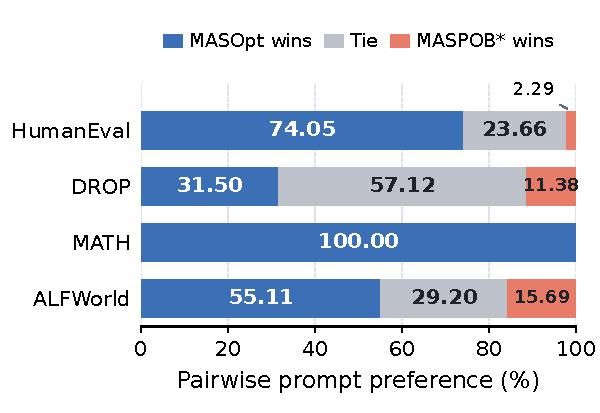
\includegraphics[width=\linewidth]{figures/prompt_quality.pdf}
        \captionsetup{width=0.98\linewidth}
        \caption{Pairwise prompt preference, with MASOpt wins, ties, and baseline wins.}
        \label{fig:prompt-quality}
    \end{minipage}\hfill
    \begin{minipage}[b]{0.285\textwidth}
        \centering
        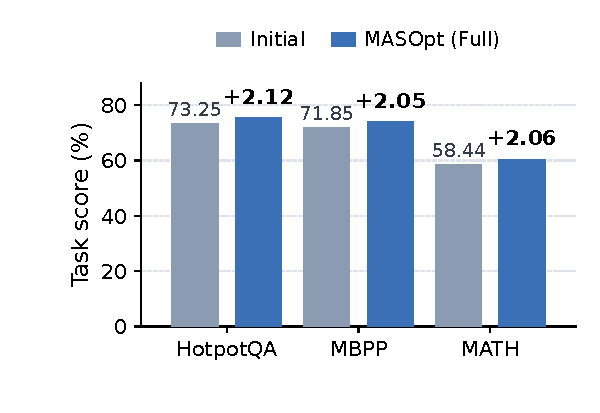
\includegraphics[width=\linewidth]{figures/architecture_adaptation.pdf}
        \captionsetup{width=0.98\linewidth}
        \caption{Adaptation to three alternative workflows, with Initial in gray and Full in blue.}
        \label{fig:architecture-adaptation}
    \end{minipage}\hfill
    \begin{minipage}[b]{0.40\textwidth}
        \centering
        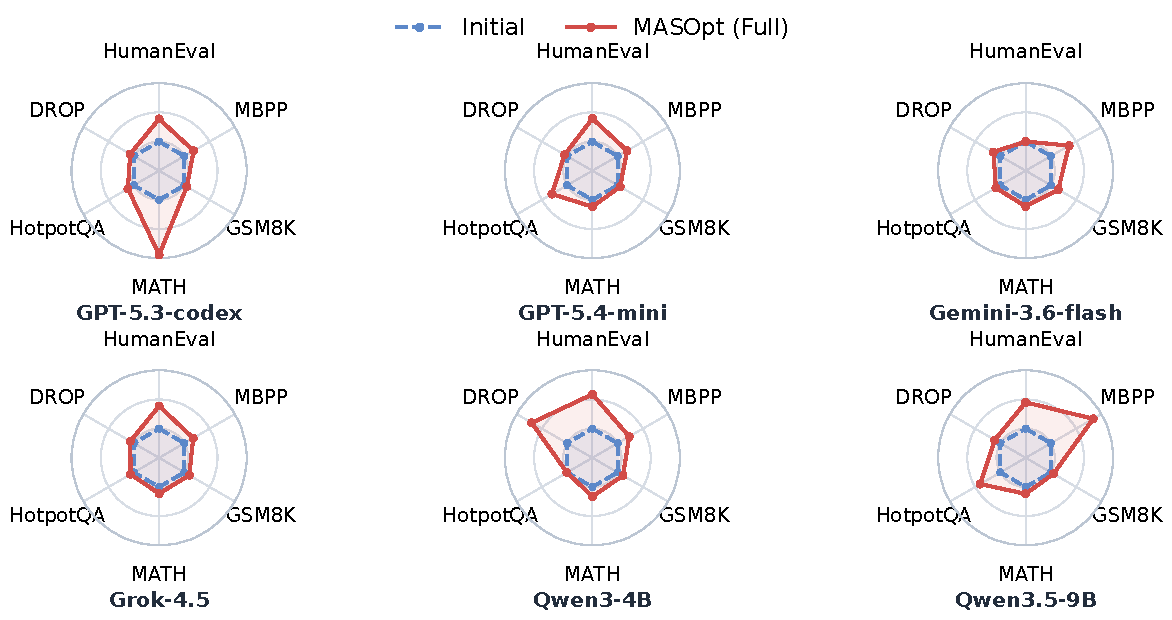
\includegraphics[width=\linewidth]{figures/backbone_radar.pdf}
        \captionsetup{width=0.98\linewidth}
        \caption{Adaptation across six backbones, with each Initial score normalized to 100.}
        \label{fig:backbone-radar}
    \end{minipage}
\end{figure}

\subsection{Advantage of the Optimized Prompts}
\label{sec:prompt-quality}

We further examine whether the closed loop improves the instructions themselves, which task accuracy alone leaves undetermined. We score the retained prompts against the offline-optimized ones under an anonymous six-dimension rubric applied in both presentation orders. As shown in Figure~\ref{fig:prompt-quality}, MASOpt is preferred on all four datasets, and the distribution across them is more informative than the aggregate, since MATH receives uniform preference while DROP is dominated by ties. This follows from what a closed loop can observe, since a MATH failure yields a derivation defect an actuation can name while a DROP repair leaves the instruction largely intact. Overall, the advantage of MASOpt appears exactly where the runtime signal is specific enough to name the defect.

\subsection{Generalizability across Workflow Architectures}
\label{sec:architecture-adaptation}

We then ask how far MASOpt depends on the workflow it repairs. Holding the backbone and the task set fixed, we rerun the identical controller on three simplified architectures. As shown in Figure~\ref{fig:architecture-adaptation}, the closed loop improves every architecture by about two points \citep{zhang2024aflow}. Overall, a controller that had learned the idiosyncrasies of the original graph would produce margins varying with the branch structure, while one acting on measured error is indifferent to it.

\subsection{Generalizability across Backbone Models}
\label{sec:backbone-adaptation}

We finally measure how the closed loop behaves under different backbones. We instantiate the identical controller on six models of different families and scales, and pair every run with its own initial workflow. As shown in Figure~\ref{fig:backbone-radar}, the paired comparison is non-negative on every model and benchmark. Notably, the single tie occurs where the initial workflow already solves the benchmark completely and leaves no failure to observe. The gate predicts this shape, since it accepts only an actuation that reduces the measured error, so a stronger backbone offers fewer opportunities to act. Overall, MASOpt transfers across model families without structural recalibration, while the size of its benefit follows how much observable failure the backbone leaves behind.

\section{Conclusion}
\label{sec:conclusion}

We introduce MASOpt, which turns MAS prompt optimization from an open-loop search into a closed-loop control problem, where a trajectory observer estimates a latent failure state, a minimal actuation repairs one prompt, and a feedback gate admits the repair only when the measured error decreases. Experiments on eight benchmarks show that MASOpt improves over the strongest offline MAS prompt optimizer on every benchmark with the backbone models and the workflow topology left fixed.

\subsection*{Ethics statement}

This work uses publicly available benchmarks and does not involve human subjects, private data, or interventions in real-world decision-making. MASOpt modifies only natural-language prompts and never updates model parameters, so its failure modes stay bounded by the behavior of the underlying models.

\subsection*{Reproducibility statement}

The formulation and the controller are specified in Section~\ref{sec:method} and the evaluation protocol in Section~\ref{sec:experiments} and Appendix~\ref{app:experimental-details}. We will release the prompt templates, the calibration trajectories, the evaluation scripts, and the configuration files needed to reproduce the reported results, subject to the terms of the underlying model and benchmark licenses.

\bibliography{iclr2027_conference}
\bibliographystyle{iclr2027_conference}

\appendix

\section{Experimental Details}
\label{app:experimental-details}

\subsection{Benchmarks}
\label{app:data-splits}

\textbf{HumanEval} \citep{chen2021humaneval} and \textbf{MBPP} \citep{austin2021mbpp} evaluate program synthesis from a natural-language specification, where a prediction is correct when it passes the hidden tests. \textbf{GSM8K} \citep{cobbe2021gsm8k} and \textbf{MATH} \citep{hendrycks2021math} evaluate multi-step mathematical reasoning, where we adopt the fixed Level-5 test subset of \citet{zhang2024aflow} that contains 155 Prealgebra, 124 Number Theory, 108 Precalculus, and 99 Counting and Probability problems. \textbf{HotpotQA} \citep{yang2018hotpotqa} evaluates multi-hop reasoning over two supporting paragraphs, and \textbf{DROP} \citep{dua2019drop} evaluates discrete reasoning that requires counting, sorting, and arithmetic over a passage. \textbf{ALFWorld} \citep{shridhar2020alfworld} evaluates embodied household tasks in a text interface with separate seen and unseen splits, and \textbf{TextCraft} \citep{prasad2024textcraft} evaluates compositional crafting in which a target item is obtained only after its recipe dependencies are satisfied in order. Success on the two interactive benchmarks therefore depends on recovering from environment feedback instead of on a single final answer, which is what makes them the setting where a closed loop has the most measurements to act on.

Table~\ref{tab:data-splits} lists the calibration pools, test sizes, and evaluation metrics of the eight benchmarks.

\begin{table}[!htbp]
    \centering
    \caption{Datasets, splits, and evaluation metrics. All reported scores are on a 0--100 scale.}
    \label{tab:data-splits}
    \small
    \setlength{\tabcolsep}{8pt}
    \begin{tabular}{@{}llrrl@{}}
        \toprule
        \textbf{Task family} & \textbf{Benchmark} & \textbf{Calibration} & \textbf{Test} & \textbf{Metric} \\
        \midrule
        \multirow{2}{*}{Code generation} & HumanEval & 33 & 131 & pass@1 \\
                        & MBPP & 86 & 341 & pass@1 \\
        \multirow{2}{*}{Mathematical reasoning} & GSM8K & 264 & 1,055 & answer accuracy \\
                               & MATH & 119 & 486 & answer accuracy \\
        \multirow{2}{*}{Reading comprehension} & HotpotQA & 200 & 800 & token F1 \\
                              & DROP & 200 & 800 & answer F1 \\
        \multirow{2}{*}{Interactive environments} & ALFWorld & 33 & 140 seen / 134 unseen & success rate \\
                                 & TextCraft & 20 & 80 & success rate \\
        \bottomrule
    \end{tabular}
\end{table}

\subsection{Baselines}
\label{app:protocols}

We compare MASOpt with three groups of methods. The first group is direct and reasoning-based prompting, covering \textbf{IO} that answers in one call, \textbf{CoT} \citep{wei2022cot} that elicits an intermediate reasoning chain, and \textbf{ReAct} \citep{yao2023react} that interleaves reasoning with tool or environment actions. The second group is prompt optimization, covering \textbf{PromptBreeder} \citep{fernando2024promptbreeder} that evolves task and mutation prompts, \textbf{Instinct} \citep{lin2023instinct} that searches instructions with a neural bandit, \textbf{MIPRO} \citep{opsahlong2024mipro} that jointly optimizes instructions and demonstrations of a language-model program, and \textbf{MASPOB} \citep{hong2026maspob} that treats fixed-topology MAS prompt optimization as budget-constrained black-box search. The third group is workflow generation and adaptation, covering \textbf{AFlow} \citep{zhang2024aflow} that searches code-represented workflows with Monte Carlo tree search and \textbf{HiveMind} \citep{xia2025hivemind} that attributes credit across agents and refines the lowest-contribution node. Baseline results on the six non-interactive benchmarks follow the evaluation setting of \citet{hong2026maspob}, and the interactive comparison uses the shared typed action interface described below.

\subsection{Implementation Protocols}
\label{app:impl}

Every agent of the target MAS is served by \texttt{gpt-4o-mini} with temperature $0$ and top-$p$ $1$, and MASOpt never updates a backbone parameter. The calibration pools listed in Table~\ref{tab:data-splits} are divided into three disjoint parts for experience construction, experience selection, and controller selection. Ground-truth rewards enter only the offline utility of Equation~\ref{eq:utility} and are never visible to the online feedback gate, which decides using the label-free measured error of Equation~\ref{eq:prompt_update} together with the deterministic runtime constraints.

On the interactive benchmarks, all compared systems use the same typed action interface, the same native environment success condition, and the same step limits of 35 on ALFWorld and 20 on TextCraft. MASOpt additionally reads the public dependency and inventory constraints that the environment exposes at every step and turns a detected violation into a bounded actuation. Its frozen controller generates task-local repairs from these public observations alone, and it neither updates the cross-task memory nor selects prompts using test accuracy.

\subsection{Measured Error}
\label{app:error}

The measured error $\mathcal{E}$ of Equation~\ref{eq:prompt_update} counts constraint violations that the runtime exposes without any label. On the code benchmarks it counts syntax errors, raised exceptions, and failures of the public tests attached to the problem statement. On the mathematical benchmarks it counts unparsable final answers, expressions that fail a symbolic well-formedness check, and disagreement among the solver branches of the workflow. On the reading benchmarks it counts answers whose span is absent from the retrieved passages, answers of the wrong type for the question, and missing fields in the message that the aggregator receives. On the interactive benchmarks it counts invalid actions rejected by the environment, actions whose preconditions are unsatisfied, and repeated states that make no progress.

Every term of $\mathcal{E}$ is a violation of a stated constraint and not an estimate of task reward, so reducing it cannot be traded against correctness the way a learned proxy can. The hidden evaluation label never enters $\mathcal{E}$, so the feedback gate of Equation~\ref{eq:accept} makes its accept and reject decisions from information that is also available at deployment.

\subsection{Analysis Protocols}
\label{app:analysis}

\textbf{Prompt quality}\quad We anonymize the prompts MASOpt retains at termination together with those the offline optimizer commits before deployment \citep{hong2026maspob}, then score both with a fixed six-dimension rubric in the two presentation orders and count a difference above $0.5$ as a win. The six dimensions cover clarity, specificity, coverage of the task constraints, handling of edge cases, compatibility with the downstream agent, and overall quality.

\textbf{Alternative architectures}\quad We replace the original graphs with one answer-generation call plus formatting on HotpotQA, one code-generation branch plus test and repair on MBPP, and two text solvers with self-consistency on MATH, then run the identical controller on each.

\subsection{Control Effort}
\label{app:cost}

We also record what the closed loop costs. We measure the total API calls of a complete TextCraft test under the shared interface and the identical 20-step limit, then compare them with the two strongest baselines. As reported in Table~\ref{tab:cost}, MASOpt uses 888 calls against 699 and 684, an increase of 27\%, and converts it into 24 solved tasks against 10 and 11. The asymmetry between the two ratios follows from Equation~\ref{eq:objective}, since no actuation is applied at a checkpoint whose measurement indicates no failure, which concentrates the budget on the episodes that would otherwise fail. Overall, the control effort scales with the number of detected failures and not with the size of the test set.

\begin{table}[!htbp]
    \centering
    \caption{Control effort and task utility on TextCraft under the shared action interface and the 20-step limit.}
    \label{tab:cost}
    \small
    \setlength{\tabcolsep}{5pt}
    \begin{tabular}{@{}lccc@{}}
        \toprule
        \textbf{Method} & \textbf{Calls} & \textbf{Solved} & \textbf{Succ.} \\
        \midrule
        \textbf{MIPRO} & 699 & 10 / 80 & 12.50 \\
        \textbf{MASPOB} & 684 & 11 / 80 & 13.75 \\
        \midrule
        \rowcolor{gray!15}\textbf{MASOpt} & 888 & \textbf{24 / 80} & \textbf{30.00} \\
        \bottomrule
    \end{tabular}
\end{table}

\subsection{Controller Hyperparameters}
\label{app:hyper}

The utility weights of Equation~\ref{eq:utility} are set so that the task-reward term dominates, with $\lambda_R = 1.0$, $\lambda_E = 0.5$, $\lambda_P = 0.3$, and $\lambda_C = 0.1$, and with $\epsilon = 10^{-6}$ in Equation~\ref{eq:cara}. The candidate set at a probed checkpoint contains the no-operation input and $K = 4$ legal local actuations. At deployment the controller retrieves the five memory entries whose failure signature best matches $s_t$ and allows at most two actuation rounds per checkpoint.

\subsection{Actuation Space}
\label{app:actuation}

The actuation space contains four types of local edit. A node-level actuation rewrites a bounded portion of the instruction of a single agent. An interface-level actuation adds a constraint on the message one agent sends to a specific downstream neighbor. A receiver-side actuation adds a rule governing how an agent consumes a message it receives. The no-operation actuation leaves the prompt state unchanged and is always available, which lets the controller decide that no repair is warranted.

\section{Case Study}
\label{app:case}

% TODO: insert one repaired trajectory here, showing the pre-actuation measurement, the diagnosed failure state, the actuation that CARA selected, and the post-actuation measurement that the gate accepted.

\end{document}
